\documentclass[11pt]{article}
\usepackage{biblatex}
\addbibresource{references.bib}
\usepackage{amsfonts,amsmath,amsthm,tikz}
\usetikzlibrary{arrows.meta,positioning}

\begin{document}
\begin{center}
\Large\textbf{Mask intervention for multi-wave epidemics}\\
\large\textit{John Bolger, Tom Falcone, Farin Rexrode}
\end{center}

\section*{Introduction}
The correlation between masking and the epidemic timeline was observed and documented during the 1918 Influenza epidemic for one of the first times. Cities around the world passed mask mandates to counter the airborne disease. In Tuscon, Arizona, the enforcement of strict masking mandates resulted in a three-fold decrease in daily influenza cases [1].
Despite the obvious effectiveness and a plethora of historical data, mask usage has faced fierce opposition across the globe, most notably with the lack of compliance with COVID-19 mask guidelines. It is crucial that public health agencies provide concise and unambiguous guidelines to optimize the number of masked individuals during an airborne epidemic, yet conflicting recommendations for mask wearing still poisons the well.

For both severe acute respiratory syndrome (SARS) and pandemic influenza, the World Health Organization (WHO) recommends wearing a mask in low-risk situations and a respirator in high-risk situations. Meanwhile, the Center for Disease Control and Prevention (CDC) recommends the use of a respirator during all human interactions that carry risk in any capacity [2]. Contradicting mask policies further damage the public's confidence in mask effectiveness, and misdirect public attention to irrelevant details. Considering a global epidemic that occurs in several waves, we should be able to use experience with previous waves to inform the response to new ones.

To serve this purpose, we will construct a classical epidemic model in which an average mask effectiveness and initial masked proportion are defined, and then determine a relationship between these values and the information of previous waves to get an epidemic threshold based on mask use. Prior knowledge of the average mask effectiveness and the basic reproduction number in the absence of mask use will reveal the minimum fraction of individuals who need to use masks preemptively to avoid another outbreak. This offers a simplistic guideline for dispersal of masking initiatives that can be expanded upon by an analysis of targeted masking and responsiveness to masking.

\section*{Model}
The population is first split into susceptible $S$, infected $I$, and recovered $R$ compartments, and then further divided into masked and unmasked individuals, indicated by a subscript of $m$ or $u$, respectively (Figure 1.). We assume that the total masked population $S_{m} + I_{m} + R_{m}$ is constant, as is the total unmasked population, and hence the total population $N$.


\begin{figure}[ht]
\begin{tikzpicture}
[node distance=3cm, auto,
    every node/.append style={align=center},
    compartment/.style={draw, minimum size=2cm}]

  \node[compartment](Su)[label=above:susceptible]{$S_{u}$};
  \node[compartment](Sm)[below=of Su]{$S_{m}$};
  \node[compartment](Iu)[right=of Su,label=above:infected]{$I_{u}$};
  \node[compartment](Im)[right=of Sm]{$I_{m}$};
  \node[compartment](Ru)[right=of Iu,label=above:recovered]{$R_{u}$};
  \node[compartment](Rm)[right=of Im]{$R_{m}$};
  \path[->] (Su) edge node {unmasked} (Iu)
  (Sm) edge node {masked} (Im)
  (Iu) edge (Ru)
  (Im) edge (Rm);
\end{tikzpicture}
\caption{Diagram with the typical SIR compartments and additional masked/unmasked subcompartments. $S_{u}$: susceptible unmasked, $S_{m}$: susceptible masked, $I_{u}$: infected unmasked, $I_{m}$: infected masked, $R_{u}$: recovered unmasked, $R_{m}$: recovered masked}
\end{figure}

\vspace{1cm}

Now, we shall derive the incidence for each interaction. Let $in_{um}$ be the incidence arising from interactions between $S_{u}$ and $I_{m}$, and similarly for any permutation of $u,m$. An \textit{adequate interaction} is an encounter between any two people that would certainly result in infection if one were susceptible, the other were infected, and both were unmasked. Let $\beta$ denote the average number of adequate interactions for one person of any compartment per unit time, and let $p$ be the probability that a mask fails to prevent infection during an adequate interaction between a susceptible and an infected. Here $p$ is assumed to be the same if only the infected is masked or only the susceptible is masked. Then one unmasked susceptible will have an average of $\beta I_{u}/N$ interactions with $I_{u}$ and $\beta p I_{m}/N$ interactions with $I_{m}$ per unit time, each of which will certainly result in infection. Similarly, one masked susceptible will face certain infection an average of $\beta p I_{u}/N$ times with $I_{u}$ and $\beta p^{2} I_{m}$ with $I_{m}$ per unit time. The resulting incidence terms are then $in_{uu} = \beta \frac{I_{u}}{N}S_{u},~in_{um} = \beta p \frac{I_{m}}{N}S_{u},~ in_{mu} = \beta p \frac{I_{u}}{N}S_{m},~in_{mm} = \beta p^{2} \frac{I_{m}}{N}S_{m}$.
Let $1/\gamma$ be the expected time spent in either infected compartment (i.e. $X \sim \text{Exp}(1/\gamma)$ models the infection time). Then our model is described by the differential equations below, where time is scaled by $1/\gamma$ and each population is scaled by $N$, (e.g. $s_{u} = S_{u}/N$).
\begin{align}
  \dot{s}_u &= - \frac{\beta }{\gamma}s_u i_u -  \frac{\beta p }{\gamma}s_u i_m \\
  \dot{s}_m &= - \frac{\beta p }{\gamma}s_m i_u -  \frac{\beta p^{2} }{\gamma} s_m i_m \\
  \dot{i}_u &=  \frac{\beta }{\gamma}s_u i_u +  \frac{\beta p }{\gamma}s_u i_m - i_u \\
  \dot{i}_m &=  \frac{\beta p }{\gamma}s_m i_u +  \frac{\beta p^{2} }{\gamma} s_m i_m - i_m\\
  \dot{r}_{u} &= i_{u}\\
  \dot{r}_{m} &= i_{m}
\end{align}
Since the total masked and unmasked populations are each constant, (5) and (6) are redundant. It is assumed that $s_0 = s_{u}(0) + s_{m}(0)$ and $i_{0} = i_{u}(0) + i_{m}(0)$ are positive, and that $r_{0} = r_{u}(0) + r_{m}(0) = 0$. The dimensionless parameters are basic reproduction numbers for simplified models: $\beta/\gamma$ if no one wears a mask, $\beta p/\gamma$ if one of $S, I$ contains only mask wearers, and the other is completely unmasked, and $\beta p^{2}/\gamma$ if everyone is masked. We proceed with a local analysis of infection free stability and derive a threshold for infectious outbreak.

\subsection*{Epidemic threshold for a new wave}
The system (5)-(10) is in equilibrium if and only if the total number of intectives $i = 0$. The Jacobian of the relevant system (5)-(8) at any fixed point $(s_{u}^*,s_{m}^*,0,0)$ is
\[
  J =
   \begin{pmatrix}
    0 & 0 & - \frac{\beta }{\gamma} s_{u}^* & - \frac{\beta p }{\gamma} s_{u}^* \\
    0 & 0 & \frac{\beta p }{\gamma} s_{m}^* & - \frac{\beta p^{2} }{\gamma} s_{m}^* \\
    0 & 0 & \frac{\beta }{\gamma} s_{u}^* - 1 & \frac{\beta p }{\gamma} s_{u}^* \\
    0 & 0 &  \frac{\beta p }{\gamma} s_{m}^* & \frac{\beta p^{2} }{\gamma} s_{m}^* - 1 \\
   \end{pmatrix}
\]
and eigenvalues are given by solutions to
\[
  \det(J - \lambda I) = \lambda^{2}\left |
  \begin{matrix}
   \frac{\beta }{\gamma} s_{u}^* - 1 - \lambda & \frac{\beta p }{\gamma} s_{u}^* \\
    \frac{\beta p }{\gamma} s_{m}^* & \frac{\beta p^{2} }{\gamma} s_{m}^* - 1 - \lambda
  \end{matrix}
  \right | = 0.
\]
The case $\lambda = 0$, corresponding to no infectives ever, can safely be ignored. Conveniently, the stability of $(s_{u}^*,s_{m}^*,0,0)$ is determined by the eigenvalues of the $2x2$ matrix
\[A =
\begin{pmatrix}
   \frac{\beta }{\gamma} s_{u}^* - 1 & \frac{\beta p }{\gamma} s_{u}^* \\
    \frac{\beta p }{\gamma} s_{m}^* & \frac{\beta p^{2} }{\gamma} s_{m}^* - 1
\end{pmatrix},
\]
for which all eigenvalues have negative real part, and hence the fixed point is stable, if and only if $\text{det} A > 0$ and $\text{tr} A < 0$. In particular, this means
\[
  1 - \frac{\beta}{\gamma}(s_{u}^{*} + p^{2}s_{m}^{*}) > 0
\]
and
\[
  \frac{\beta}{\gamma}(s_{u}^{*} + p^{2}s_{m}^{*}) < 2.
\]
Let $P_{o} = \frac{\beta}{\gamma}$, the prior basic reproduction number determined from a previous wave in an unmasked population. If the threat of a new wave is introduced to a wholly susceptible population via a single infected, we have $s_{m}^* = s_{m}(0) = f$ and $s_{u}^* = s_{u}(0) = 1-f$, where f is the fraction of all people that wear masks. Let $R_{o} =   P_{o}(1 - f + p^{2}f) = P_{o}(1 + (m^{2}-2m)f)$, where $m = 1 - p$ is the probability that a mask blocks infection. Intuitively, $R_{o}$ is the average number of secondary infections in a wholly susceptible population caused by a lone infected person who mirrors the masking habits of each susceptible. Indeed $R_{o}$ satisfies the typical properties of a basic reproduction number~\cite{martcheva2015introduction}.
The above inequalities are both satisfied, and hence an epidemic is avoided, if and only if $R_{o} < 1$, which is to say less than a single infection arises in the foregoing scenario. To facilitate social guidance, the relevant data here are $P_{o}, f,$ and $m,$ which are implicit in the threshold condition:
\begin{equation}
  R_{o} < 1 \iff 1+(m^{2} - 2m) f < \frac{1}{P_{o}} \iff (2m - m^{2})f > 1 - \frac{1}{P_{o}}.
\end{equation}
So, given $m$ and $P_{o}$, infectious outbreak won't occur for $f > \frac{P_{o}-1}{P_{o}(2m - m^{2})}$. Depending on the size of the right hand side, a judgement can be made by public health officals to determine how involved masking will be as an intervention, and whether mandates should be sought to put more of the burden on masking rather than costlier interventions like contact tracing, pharmaceuticals, or quarantine. The advice should always be to wear the best quality masks as much as possible, so the relevance of our threshold is in the determination of how much time and money is spent to disperse this message with respect to other interventions.

\section*{Example: Early COVID-19}
In 2020, the value of $P_{o}$ for COVID-19 was estimated to be roughly equal to $3.5$~\cite{alimohamadi2020estimate}\cite{howard2021evidence}. In addition, we can use the estimated infectious period of 15.2 days~\cite{van2021duration} to plot the day-wise evolution of a potential new wave of COVID-19 for values that satisfy (7) and those that don't (Figure. 2). Assuming that the average mask is a surgical mask, we have $m = 0.9$~\cite{morais2021filtration}, and so $\frac{P_{o}-1}{P_{o}(2m - m^{2})} = 0.7215$. The epidemic disappears for $f > 0.7215$.
\begin{figure}[ht]
  \centering
  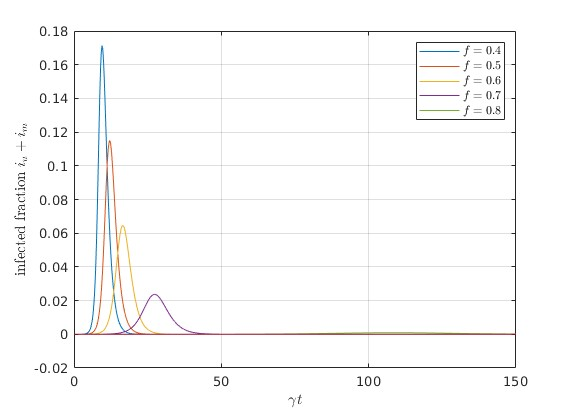
\includegraphics[width=11.0cm]{fvals.jpg}
  \caption{\label{fig:11sat} Total infected fraction in $1/\gamma$ scaled time $\tau$. }
\end{figure}

\section*{Proposed work}
We will further analyze the effectiveness of mask use in the context of a renewal process with latent $L$, pre-symptomatic and pre-peak infectiousness $A_{1}$, pre-symptomatic and post-peak infectiousness $A_{2}$, and symptomatic $S$ stages~\cite{tian2021harnessing}. How does altering mask use at different stages of exposure compare to a universal masking habit? Dependent on the time $t_{L}$ spent in $L$, the transfer rate from $L$ to $A_{1}$ is $\alpha_{L}(t_{L})$. The waiting time between $A_{1}$ to $A_{2}$ is random $X \sim \text{Exp}(1/\alpha_{A})$, and a constant time $t_{P}$ is spent between $A_{2}$ and $S$. To capture any new infections, we have the transmission rates $\beta_{A_{1}}$, $\beta_{A_{2}}$, and $\beta_{S}$ from the infectious states into $L$, each of which possibly varies with time. Our study will focus on the development of an epidemic when these transmission rates are damped by masking functions $m_{A_{1}}, m_{A_{2}}, m_{S}$ which vary in time according to the proportion of individuals masked in the corresponding state. This will inform a targeted masking policy that accounts for population response.

\printbibliography

\end{document}
